\documentclass[sigconf,nonacm]{acmart}
% BOMwitness, SafeIoT Hackathon 2026, Track 2.
% Every result number below is a macro from numbers.tex, which gen_numbers.py derives from results/r2/.
% check_numbers.py fails the build if a number in the PDF is not accounted for.
\usepackage{booktabs}
\usepackage{tikz}
\usetikzlibrary{positioning,arrows.meta,fit,calc}
\usepackage{pgfplots}
\pgfplotsset{compat=1.17}
% generated by paper/gen_numbers.py from the committed result files; do not edit
\newcommand{\nHeldImages}{10}
\newcommand{\nTuneImages}{4}
\newcommand{\nImages}{14}
\newcommand{\nArchHeld}{6}
\newcommand{\nArchAll}{7}
\newcommand{\nTargetsHeld}{10}
\newcommand{\nHeldCases}{1,860}
\newcommand{\nTuneCases}{744}
\newcommand{\nAllCases}{2,604}
\newcommand{\nDistinctErr}{900}
\newcommand{\nAllDistinctErr}{1,260}
\newcommand{\kPerClass}{12}
\newcommand{\seed}{20261127}
\newcommand{\freezeCommit}{0f83a98}
\newcommand{\bomtraceCommit}{64e5264}
\newcommand{\nBomErrCases}{480}
\newcommand{\nUnawareCases}{420}
\newcommand{\nBomRows}{1,440}
\newcommand{\nAllBomRows}{2,016}
\newcommand{\nAllUnawareRows}{588}
\newcommand{\nMFourUCases}{60}
\newcommand{\kUnindexed}{6}
\newcommand{\pHonFo}{0.993}
\newcommand{\rHonFo}{0.867}
\newcommand{\tpHonFo}{416}
\newcommand{\pHonNs}{0.994}
\newcommand{\rHonNs}{0.979}
\newcommand{\tpHonNs}{470}
\newcommand{\pHonBw}{0.994}
\newcommand{\rHonBw}{0.988}
\newcommand{\tpHonBw}{474}
\newcommand{\pHonBt}{1.000}
\newcommand{\rHonBt}{1.000}
\newcommand{\tpHonBt}{480}
\newcommand{\pHonSy}{0.442}
\newcommand{\rHonSy}{1.000}
\newcommand{\tpHonSy}{480}
\newcommand{\pHonCv}{0.342}
\newcommand{\rHonCv}{0.027}
\newcommand{\tpHonCv}{13}
\newcommand{\casesHon}{480}
\newcommand{\pColFo}{0.993}
\newcommand{\rColFo}{0.867}
\newcommand{\tpColFo}{416}
\newcommand{\pColNs}{0.994}
\newcommand{\rColNs}{0.979}
\newcommand{\tpColNs}{470}
\newcommand{\pColBw}{0.994}
\newcommand{\rColBw}{0.988}
\newcommand{\tpColBw}{474}
\newcommand{\rColBt}{0.000}
\newcommand{\tpColBt}{0}
\newcommand{\pColSy}{0.000}
\newcommand{\rColSy}{0.000}
\newcommand{\tpColSy}{0}
\newcommand{\pColCv}{0.342}
\newcommand{\rColCv}{0.027}
\newcommand{\tpColCv}{13}
\newcommand{\casesCol}{480}
\newcommand{\pStrFo}{0.993}
\newcommand{\rStrFo}{0.867}
\newcommand{\tpStrFo}{416}
\newcommand{\pStrNs}{0.994}
\newcommand{\rStrNs}{0.979}
\newcommand{\tpStrNs}{470}
\newcommand{\pStrBw}{0.994}
\newcommand{\rStrBw}{0.988}
\newcommand{\tpStrBw}{474}
\newcommand{\rStrBt}{0.000}
\newcommand{\tpStrBt}{0}
\newcommand{\pStrSy}{0.055}
\newcommand{\rStrSy}{0.250}
\newcommand{\tpStrSy}{120}
\newcommand{\pStrCv}{0.342}
\newcommand{\rStrCv}{0.027}
\newcommand{\tpStrCv}{13}
\newcommand{\casesStr}{480}
\newcommand{\pUnaFo}{0.993}
\newcommand{\rUnaFo}{0.945}
\newcommand{\tpUnaFo}{397}
\newcommand{\pUnaNs}{0.993}
\newcommand{\rUnaNs}{0.945}
\newcommand{\tpUnaNs}{397}
\newcommand{\pUnaBw}{0.993}
\newcommand{\rUnaBw}{0.955}
\newcommand{\tpUnaBw}{401}
\newcommand{\rUnaBt}{0.000}
\newcommand{\tpUnaBt}{0}
\newcommand{\pUnaSy}{0.000}
\newcommand{\rUnaSy}{0.000}
\newcommand{\tpUnaSy}{0}
\newcommand{\pUnaCv}{0.365}
\newcommand{\rUnaCv}{0.055}
\newcommand{\tpUnaCv}{23}
\newcommand{\casesUna}{420}
\newcommand{\pAllFo}{0.993}
\newcommand{\rAllFo}{0.884}
\newcommand{\tpAllFo}{1,645}
\newcommand{\pAllNs}{0.993}
\newcommand{\rAllNs}{0.972}
\newcommand{\tpAllNs}{1,807}
\newcommand{\pAllBw}{0.994}
\newcommand{\rAllBw}{0.980}
\newcommand{\tpAllBw}{1,823}
\newcommand{\pAllBt}{1.000}
\newcommand{\rAllBt}{0.258}
\newcommand{\tpAllBt}{480}
\newcommand{\pAllSy}{0.134}
\newcommand{\rAllSy}{0.323}
\newcommand{\tpAllSy}{600}
\newcommand{\pAllCv}{0.350}
\newcommand{\rAllCv}{0.033}
\newcommand{\tpAllCv}{62}
\newcommand{\casesAll}{1,860}
\newcommand{\loColBw}{0.973}
\newcommand{\hiColBw}{0.994}
\newcommand{\minColBw}{0.958}
\newcommand{\loColNs}{0.962}
\newcommand{\hiColNs}{0.989}
\newcommand{\minColNs}{0.958}
\newcommand{\loColFo}{0.833}
\newcommand{\hiColFo}{0.894}
\newcommand{\minColFo}{0.771}
\newcommand{\loUnaBw}{0.930}
\newcommand{\hiUnaBw}{0.971}
\newcommand{\minUnaBw}{0.929}
\newcommand{\loUnaNs}{0.919}
\newcommand{\hiUnaNs}{0.963}
\newcommand{\minUnaNs}{0.881}
\newcommand{\loUnaFo}{0.919}
\newcommand{\hiUnaFo}{0.963}
\newcommand{\minUnaFo}{0.881}
\newcommand{\imgMinColBw}{0.958}
\newcommand{\imgMaxColBw}{1.000}
\newcommand{\imgMedColBw}{0.990}
\newcommand{\imgPerfectColBw}{5}
\newcommand{\imgMinColNs}{0.958}
\newcommand{\imgMaxColNs}{1.000}
\newcommand{\imgMedColNs}{0.979}
\newcommand{\imgPerfectColNs}{3}
\newcommand{\imgMinColFo}{0.771}
\newcommand{\imgMaxColFo}{0.958}
\newcommand{\imgMedColFo}{0.875}
\newcommand{\imgPerfectColFo}{0}
\newcommand{\imgMinUnaBw}{0.929}
\newcommand{\imgMaxUnaBw}{0.976}
\newcommand{\imgMedUnaBw}{0.952}
\newcommand{\imgPerfectUnaBw}{0}
\newcommand{\imgMinUnaNs}{0.881}
\newcommand{\imgMaxUnaNs}{0.976}
\newcommand{\imgMedUnaNs}{0.952}
\newcommand{\imgPerfectUnaNs}{0}
\newcommand{\imgMinUnaFo}{0.881}
\newcommand{\imgMaxUnaFo}{0.976}
\newcommand{\imgMedUnaFo}{0.952}
\newcommand{\imgPerfectUnaFo}{0}
\newcommand{\btStrNoResult}{480}
\newcommand{\btColRan}{480}
\newcommand{\syStrCredited}{120}
\newcommand{\caseFp}{0}
\newcommand{\nErrFalsePositives}{0}
\newcommand{\rColAo}{0.988}
\newcommand{\tpColAo}{474}
\newcommand{\pColAo}{0.994}
\newcommand{\rColBo}{0.619}
\newcommand{\tpColBo}{297}
\newcommand{\pColBo}{1.000}
\newcommand{\tpHonWithDb}{480}
\newcommand{\rHonWithDb}{1.000}
\newcommand{\rUnaBo}{0.383}
\newcommand{\pColNoNorm}{0.988}
\newcommand{\cleanFpNoNorm}{6}
\newcommand{\kMOneFo}{120}
\newcommand{\kMOneNs}{120}
\newcommand{\kMOneBw}{120}
\newcommand{\kMOneCases}{120}
\newcommand{\kMOneBtHon}{120}
\newcommand{\kMOneBtCol}{0}
\newcommand{\kMOneBtStr}{0}
\newcommand{\kMOneSyHon}{120}
\newcommand{\kMOneSyCol}{0}
\newcommand{\kMOneSyStr}{0}
\newcommand{\kMOneCvHon}{5}
\newcommand{\kMOneCvCol}{5}
\newcommand{\kMOneCvStr}{5}
\newcommand{\kMTwoFo}{119}
\newcommand{\kMTwoNs}{119}
\newcommand{\kMTwoBw}{120}
\newcommand{\kMTwoCases}{120}
\newcommand{\kMTwoBtHon}{120}
\newcommand{\kMTwoBtCol}{0}
\newcommand{\kMTwoBtStr}{0}
\newcommand{\kMTwoSyHon}{120}
\newcommand{\kMTwoSyCol}{0}
\newcommand{\kMTwoSyStr}{0}
\newcommand{\kMTwoCvHon}{6}
\newcommand{\kMTwoCvCol}{6}
\newcommand{\kMTwoCvStr}{6}
\newcommand{\kMTwoBFo}{60}
\newcommand{\kMTwoBNs}{114}
\newcommand{\kMTwoBBw}{117}
\newcommand{\kMTwoBCases}{120}
\newcommand{\kMTwoBBtHon}{120}
\newcommand{\kMTwoBBtCol}{0}
\newcommand{\kMTwoBBtStr}{0}
\newcommand{\kMTwoBSyHon}{120}
\newcommand{\kMTwoBSyCol}{0}
\newcommand{\kMTwoBSyStr}{0}
\newcommand{\kMTwoBCvHon}{2}
\newcommand{\kMTwoBCvCol}{2}
\newcommand{\kMTwoBCvStr}{2}
\newcommand{\kMThreeFo}{117}
\newcommand{\kMThreeNs}{117}
\newcommand{\kMThreeBw}{117}
\newcommand{\kMThreeCases}{120}
\newcommand{\kMThreeBtHon}{120}
\newcommand{\kMThreeBtCol}{0}
\newcommand{\kMThreeBtStr}{0}
\newcommand{\kMThreeSyHon}{120}
\newcommand{\kMThreeSyCol}{0}
\newcommand{\kMThreeSyStr}{120}
\newcommand{\kMThreeCvHon}{0}
\newcommand{\kMThreeCvCol}{0}
\newcommand{\kMThreeCvStr}{0}
\newcommand{\kMFourFo}{120}
\newcommand{\kMFourNs}{120}
\newcommand{\kMFourBw}{120}
\newcommand{\kMFourCases}{120}
\newcommand{\kMFourBtUna}{0}
\newcommand{\kMFourSyUna}{0}
\newcommand{\kMFourCvUna}{8}
\newcommand{\kMFourUFo}{41}
\newcommand{\kMFourUNs}{41}
\newcommand{\kMFourUBw}{41}
\newcommand{\kMFourUCases}{60}
\newcommand{\kMFourUBtUna}{0}
\newcommand{\kMFourUSyUna}{0}
\newcommand{\kMFourUCvUna}{6}
\newcommand{\kMFiveFo}{120}
\newcommand{\kMFiveNs}{120}
\newcommand{\kMFiveBw}{120}
\newcommand{\kMFiveCases}{120}
\newcommand{\kMFiveBtUna}{0}
\newcommand{\kMFiveSyUna}{0}
\newcommand{\kMFiveCvUna}{9}
\newcommand{\kMSixFo}{116}
\newcommand{\kMSixNs}{116}
\newcommand{\kMSixBw}{120}
\newcommand{\kMSixCases}{120}
\newcommand{\kMSixBtUna}{0}
\newcommand{\kMSixSyUna}{0}
\newcommand{\kMSixCvUna}{0}
\newcommand{\patchMissNoSnap}{4}
\newcommand{\nAlgPatterns}{19}
\newcommand{\cleanDeclared}{1,470}
\newcommand{\cleanVerA}{1,348}
\newcommand{\cleanVerAPct}{91.7}
\newcommand{\cleanVerB}{23}
\newcommand{\cleanUnver}{96}
\newcommand{\cleanAlarms}{3}
\newcommand{\cleanAlarmPct}{0.20}
\newcommand{\cleanFiles}{6,135}
\newcommand{\cleanAccounted}{6,134}
\newcommand{\cleanCode}{1,582}
\newcommand{\cleanCodeAccounted}{1,582}
\newcommand{\cleanUnverMeta}{93}
\newcommand{\cleanUnverMoved}{3}
\newcommand{\syftCleanMin}{44}
\newcommand{\syftCleanMax}{76}
\newcommand{\syftCleanStrMin}{158}
\newcommand{\syftCleanStrMax}{251}
\newcommand{\cleanPassPct}{93.3}
\newcommand{\cleanUnverPct}{6.5}
\newcommand{\exDeclared}{150}
\newcommand{\exPass}{139}
\newcommand{\exFail}{4}
\newcommand{\exFailDeclared}{3}
\newcommand{\exReview}{0}
\newcommand{\exUnver}{8}
\newcommand{\exFiles}{629}
\newcommand{\exFilesAccounted}{629}
\newcommand{\exDeprecated}{31}
\newcommand{\exDbDisagree}{4}
\newcommand{\nMisses}{25}
\newcommand{\missImplant}{19}
\newcommand{\missPhantom}{3}
\newcommand{\missFabricated}{3}
\newcommand{\tuneColR}{1.000}
\newcommand{\tuneColTp}{192}
\newcommand{\tuneColCases}{192}
\newcommand{\tuneUnaR}{0.964}
\newcommand{\tuneUnaTp}{162}
\newcommand{\tuneUnaCases}{168}
\newcommand{\farImages}{7}
\newcommand{\farColR}{0.988}
\newcommand{\farColP}{1.000}
\newcommand{\farColTp}{332}
\newcommand{\farColCases}{336}
\newcommand{\farUnaR}{0.963}
\newcommand{\farUnaP}{1.000}
\newcommand{\farUnaTp}{283}
\newcommand{\farUnaCases}{294}
\newcommand{\sibHave}{11}
\newcommand{\sibTwins}{8}
\newcommand{\sibRest}{3}
\newcommand{\sibRestMinPct}{99.5}
\newcommand{\sibRestMaxPct}{99.9}
\newcommand{\sibNone}{3}
\newcommand{\wideImages}{2}
\newcommand{\wideAfter}{12}
\newcommand{\wideBefore}{9}
\newcommand{\wideCases}{12}
\newcommand{\wideMbMin}{390}
\newcommand{\wideMbMax}{400}
\newcommand{\cbomImages}{14}
\newcommand{\cbomClasses}{15}
\newcommand{\cbomCases}{994}
\newcommand{\cbomTp}{1,272}
\newcommand{\cbomExpected}{1,274}
\newcommand{\cbomMissed}{2}
\newcommand{\cbomExtra}{0}
\newcommand{\driftReleases}{15}
\newcommand{\driftOldTwentyFourAge}{661}
\newcommand{\driftOldTwentyFourFo}{58.7}
\newcommand{\driftOldTwentyFourFoAlarms}{3}
\newcommand{\driftOldTwentyFourMa}{63.3}
\newcommand{\driftOldTwentyFourMaAlarms}{3}
\newcommand{\driftOldTwentyFourSn}{93.3}
\newcommand{\driftOldTwentyFourSnAlarms}{0}
\newcommand{\driftOldTwentyFourRelabelled}{53}
\newcommand{\driftOldTwentyFourDeclared}{150}
\newcommand{\driftNewTwentyFourAge}{126}
\newcommand{\driftNewTwentyFourFo}{80.0}
\newcommand{\driftNewTwentyFourFoAlarms}{0}
\newcommand{\driftNewTwentyFourMa}{89.3}
\newcommand{\driftNewTwentyFourMaAlarms}{0}
\newcommand{\driftNewTwentyFourSn}{93.3}
\newcommand{\driftNewTwentyFourSnAlarms}{0}
\newcommand{\driftNewTwentyFourRelabelled}{24}
\newcommand{\driftNewTwentyFourDeclared}{150}
\newcommand{\driftOldTwentyThreeAge}{1,144}
\newcommand{\driftOldTwentyThreeFo}{67.8}
\newcommand{\driftOldTwentyThreeFoAlarms}{5}
\newcommand{\driftOldTwentyThreeMa}{69.9}
\newcommand{\driftOldTwentyThreeMaAlarms}{5}
\newcommand{\driftOldTwentyThreeSn}{92.5}
\newcommand{\driftOldTwentyThreeSnAlarms}{1}
\newcommand{\driftOldTwentyThreeRelabelled}{36}
\newcommand{\driftOldTwentyThreeDeclared}{146}
\newcommand{\driftNewTwentyThreeAge}{469}
\newcommand{\driftNewTwentyThreeFo}{93.2}
\newcommand{\driftNewTwentyThreeFoAlarms}{0}
\newcommand{\driftNewTwentyThreeMa}{93.2}
\newcommand{\driftNewTwentyThreeMaAlarms}{0}
\newcommand{\driftNewTwentyThreeSn}{93.2}
\newcommand{\driftNewTwentyThreeSnAlarms}{0}
\newcommand{\driftNewTwentyThreeRelabelled}{0}
\newcommand{\driftNewTwentyThreeDeclared}{146}
\newcommand{\driftSnapAlarmsTotal}{1}
\newcommand{\driftFeedAlarmsTotal}{35}
\newcommand{\driftSnapMinPct}{92.5}
\newcommand{\driftSnapMaxPct}{93.3}
\newcommand{\republishedTwentyFourPct}{31.4}
\newcommand{\republishedTwentyFour}{219}
\newcommand{\baseFeedTwentyFour}{697}
\newcommand{\republishedTwentyThreePct}{8.5}
\newcommand{\republishedTwentyThree}{57}
\newcommand{\baseFeedTwentyThree}{670}
\newcommand{\obImages}{14}
\newcommand{\obClaims}{1,868}
\newcommand{\obVerified}{1,705}
\newcommand{\obWrongVersion}{34}
\newcommand{\obWrongVersionImages}{7}
\newcommand{\obAbsent}{3}
\newcommand{\obUnverifiable}{122}
\newcommand{\obBytesDiffer}{4}
\newcommand{\obVerA}{1,674}
\newcommand{\obVerB}{31}
\newcommand{\obBeyondMin}{0}
\newcommand{\obBeyondMax}{45}
\newcommand{\obBeyondTotal}{211}
\newcommand{\obBeyondImages}{11}
\newcommand{\obBeyondFiles}{477}
\newcommand{\obOrphanCode}{0}
\newcommand{\invNamed}{1,939}
\newcommand{\invInstalled}{1,950}
\newcommand{\invInstalledAll}{2,083}
\newcommand{\invWrong}{0}
\newcommand{\invSyftMin}{45}
\newcommand{\invSyftMax}{77}
\newcommand{\invCveMin}{6}
\newcommand{\invCveMax}{11}
\newcommand{\forkRelease}{24.10.7}
\newcommand{\forkDeclared}{190}
\newcommand{\forkOwnVerified}{183}
\newcommand{\forkOwnFindings}{0}
\newcommand{\forkOwnUnver}{7}
\newcommand{\forkUpVerA}{74}
\newcommand{\forkUpVerAPct}{39}
\newcommand{\forkUpWrongVersion}{55}
\newcommand{\forkUpBytesDiffer}{17}
\newcommand{\forkUpAbsent}{9}
\newcommand{\forkUpOrphans}{110}
\newcommand{\forkExeSame}{65}
\newcommand{\forkExeTotal}{215}
\newcommand{\forkFilesSame}{480}
\newcommand{\forkFilesTotal}{830}
\newcommand{\forkOmitted}{5}
\newcommand{\forkOmittedFound}{5}
\newcommand{\secMin}{0.05}
\newcommand{\secMax}{0.11}
\newcommand{\secBomtrace}{0.07}
\newcommand{\secSyft}{1.0}
\newcommand{\eTwoEWarm}{5.2}
\newcommand{\eTwoECold}{13.7}
\newcommand{\indexSecMin}{29}
\newcommand{\indexSecMax}{40}
\newcommand{\indexMbMin}{149}
\newcommand{\indexMbMax}{197}
\newcommand{\indexGbTotal}{2.1}
\newcommand{\indexTargets}{14}
\newcommand{\indexPkgsMin}{1,839}
\newcommand{\indexPkgsMax}{2,086}
\newcommand{\postImages}{3}
\newcommand{\postCases}{558}
\newcommand{\postDiffs}{0}
\newcommand{\verdictCheckImages}{14}
\newcommand{\verdictCheckCases}{2,604}
\newcommand{\verdictCheckDiffs}{0}
\newcommand{\verdictRecheckImages}{14}
\newcommand{\verdictRecheckCases}{2,604}
\newcommand{\verdictRecheckDiffs}{0}

% generated by gen_numbers.py from results/r2/drift.json
\def\driftticks{23.05.0,23.05.2,23.05.3,23.05.4,23.05.5,23.05.6,24.10.0,24.10.1,24.10.2,24.10.3,24.10.4,24.10.5,24.10.6,24.10.7,24.10.8}
\def\driftticklabels{.0,.2,.3,.4,.5,.6,.0,.1,.2,.3,.4,.5,.6,.7,.8}
\def\driftplots{%
\addplot[black, mark=o, mark size=1.3pt, densely dashed] coordinates {(23.05.0,67.8) (23.05.2,71.9) (23.05.3,74.0) (23.05.4,76.0) (23.05.5,83.6) (23.05.6,93.2)};
\addlegendentry{feeds only}
\addplot[black, mark=o, mark size=1.3pt, densely dashed, forget plot] coordinates {(24.10.0,58.7) (24.10.1,59.3) (24.10.2,60.7) (24.10.3,64.0) (24.10.4,66.0) (24.10.5,66.7) (24.10.6,69.3) (24.10.7,70.7) (24.10.8,80.0)};
\addplot[black, mark=triangle*, mark size=1.5pt] coordinates {(23.05.0,69.9) (23.05.2,74.7) (23.05.3,77.4) (23.05.4,84.9) (23.05.5,86.3) (23.05.6,93.2)};
\addlegendentry{+ signed manifest}
\addplot[black, mark=triangle*, mark size=1.5pt, forget plot] coordinates {(24.10.0,63.3) (24.10.1,66.7) (24.10.2,69.3) (24.10.3,72.7) (24.10.4,74.0) (24.10.5,75.3) (24.10.6,78.7) (24.10.7,80.0) (24.10.8,89.3)};
\addplot[black, mark=square*, mark size=1.1pt, thick] coordinates {(23.05.0,92.5) (23.05.2,93.2) (23.05.3,93.2) (23.05.4,93.2) (23.05.5,93.2) (23.05.6,93.2)};
\addlegendentry{+ sibling snapshot}
\addplot[black, mark=square*, mark size=1.1pt, thick, forget plot] coordinates {(24.10.0,93.3) (24.10.1,93.3) (24.10.2,93.3) (24.10.3,93.3) (24.10.4,93.3) (24.10.5,93.3) (24.10.6,93.3) (24.10.7,93.3) (24.10.8,93.3)};
}

% generated by gen_numbers.py
\def\tabmainrows{%
honest & 480 & 0.993 / 0.867 & 0.994 / 0.979 & 0.994 / 0.988 & 1.000 / 1.000 & 0.442 / 1.000 & 0.342 / 0.027 \\
colluding & 480 & 0.993 / 0.867 & 0.994 / 0.979 & 0.994 / 0.988 & n/a / 0.000 & 0.000 / 0.000 & 0.342 / 0.027 \\
stripped & 480 & 0.993 / 0.867 & 0.994 / 0.979 & 0.994 / 0.988 & n/a / 0.000 & 0.055 / 0.250 & 0.342 / 0.027 \\
unaware & 420 & 0.993 / 0.945 & 0.993 / 0.945 & 0.993 / 0.955 & n/a / 0.000 & 0.000 / 0.000 & 0.365 / 0.055 \\
\midrule
all cases & 1,860 & 0.993 / 0.884 & 0.993 / 0.972 & 0.994 / 0.980 & 1.000 / 0.258 & 0.134 / 0.323 & 0.350 / 0.033 \\
}

% generated by gen_numbers.py
\def\tabclassrows{%
M1 & omitted & 120 & 120 & 120 & 120 & 120 / 0 / 0 & 120 / 0 / 0 & 5 / 5 / 5 \\
M2 & other-release version & 120 & 119 & 119 & 120 & 120 / 0 / 0 & 120 / 0 / 0 & 6 / 6 / 6 \\
M2b & fabricated version & 120 & 60 & 114 & 117 & 120 / 0 / 0 & 120 / 0 / 0 & 2 / 2 / 2 \\
M3 & phantom & 120 & 117 & 117 & 117 & 120 / 0 / 0 & 120 / 0 / 120 & 0 / 0 / 0 \\
M4 & implant & 120 & 120 & 120 & 120 & 0 & 0 & 8 \\
M4u & implant, unindexed & 60 & 41 & 41 & 41 & 0 & 0 & 6 \\
M5 & swapped binary & 120 & 120 & 120 & 120 & 0 & 0 & 9 \\
M6 & patched byte & 120 & 116 & 116 & 120 & 0 & 0 & 0 \\
}

% generated by gen_numbers.py from pipeline/4_analysis_output/bomwitness/report-with-errors.json
\def\tabexamplerows{%
SBOM & \vd{wrong\_version} & busybox & A & declared 1.36.2-r3; bytes are the publisher's build 1.36.1-r3 \\
SBOM & \vd{wrong\_version} & dropbear & A & declared 2022.82-6; bytes are the publisher's build 2024.86-r3 \\
SBOM & \vd{absent} & tcpdump & A & no file of the reference package is in the image \\
SBOM & \vd{undeclared\_component} & dnsmasq & A & 12 files byte-identical to dnsmasq 2.93-r1, not in the BOM \\
CBOM & \vd{undeclared\_certificate} & certificate DigiCert TLS ECC P384 Root G5 & A & in the image's CA bundle, not in the CBOM \\
cross & \vd{provider\_unverified} & busybox & A & CBOM names it as provider of MD5, but its SBOM check ended in \vd{wrong\_version} \\
cross & \vd{provider\_unverified} & dropbear & A & CBOM names it as provider of AES, but its SBOM check ended in \vd{wrong\_version} \\
cross & \vd{algorithm\_not\_evidenced} & ML-KEM in libmbedtls21 & B & no file of the named provider carries the algorithm's name \\
}

% generated by gen_numbers.py
\def\tabimagerows{%
edgerouter-x & 23.05.6 & mipsel\_24kc & 114 & 105 & 2 & 7 & 0 & twin \\
gl-b1300 & 23.05.6 & arm\_cortex-a7\_neon-vfpv4 & 144 & 134 & 2 & 8 & 0 & twin \\
gl-mt3000 & 23.05.6 & aarch64\_cortex-a53 & 155 & 143 & 2 & 10 & 0 & 99.7\% \\
rpi-4 & 23.05.6 & aarch64\_cortex-a72 & 157 & 143 & 2 & 11 & 1 & none \\
x86-64 & 23.05.6 & x86\_64 & 150 & 134 & 2 & 13 & 1 & none \\
archer-c50-v4 & 24.10.8 & mipsel\_24kc & 140 & 131 & 2 & 7 & 0 & twin \\
gl-b1300 & 24.10.8 & arm\_cortex-a7\_neon-vfpv4 & 148 & 138 & 2 & 8 & 0 & twin \\
unifi-6-lr-v1 & 24.10.8 & aarch64\_cortex-a53 & 149 & 138 & 2 & 9 & 0 & 99.5\% \\
wrt1900acs & 24.10.8 & arm\_cortex-a9\_vfpv3-d16 & 138 & 129 & 2 & 7 & 0 & twin \\
x86-64 & 24.10.8 & x86\_64 & 175 & 153 & 5 & 16 & 1 & none \\
}

\newcommand{\tool}{BOMwitness}
\newcommand{\ubreak}{\textunderscore\allowbreak}
\newcommand{\vd}[1]{{\ttfamily\let\_\ubreak #1}}
\emergencystretch=1.2em
\setlength{\textfloatsep}{8pt plus 2pt minus 2pt}
\setlength{\floatsep}{6pt plus 2pt minus 2pt}
\setlength{\dbltextfloatsep}{8pt plus 2pt minus 2pt}

\begin{document}

\title{BOMwitness: Verifying IoT Firmware Bills of Materials Against the Bytes, Not the Device's Own Package Database}

\author{Andrew Winton}
\affiliation{\institution{Independent}\country{USA}}

\begin{abstract}
Open tools that check a software bill of materials (SBOM) for Linux-based IoT firmware take their inventory from the package database inside the firmware, so they compare the BOM with the device's own self-report. We show what that costs. On \nHeldImages{} held-out official OpenWrt images with \nHeldCases{} seeded single errors, a published database-reading verifier and a diff built on a popular SBOM generator find every BOM-level error when the database is honest, none when it agrees with the wrong BOM, at most a recall of \rStrSy{} when it has been stripped, and no implanted, swapped or patched binary in any condition. \tool{} instead checks each SBOM and CBOM claim against the publisher's signed release material and grades the evidence. Using signed package feeds alone it keeps precision \pColFo{} and recall \rColFo{} in all three database conditions; a signed release manifest raises recall to \rColNs{}. We answer directly why such numbers are easy by construction, measure how the reference decays as feeds are rebuilt, verify OpenWrt's own published BOMs (\obWrongVersion{} contradicted version claims), and show on a downstream fork where byte identity stops. Code, benchmark and results are open source.
\end{abstract}

\keywords{SBOM, CBOM, AI-BOM, firmware, IoT, supply-chain security, verification, OpenWrt}

\maketitle

\section{Introduction}

Software bills of materials are becoming something a buyer or regulator can demand \cite{ntia2021minimum,cra2024}, and NIST's consumer IoT baseline asks developers to document cybersecurity-relevant information about a product and its components \cite{nistir8425}. A BOM that nobody checks is a claim, and studies report that generated BOMs are often inconsistent or incomplete and that practitioners doubt their accuracy \cite{yu2024correctness,balliu2023challenges,xia2023empirical,stalnaker2024boms}. For compiled firmware the checking is hard: the artifact is a flash image, not a dependency manifest.

The open tools that handle Linux firmware get around this by reading the package database that ships inside the image (the opkg \texttt{status} file on OpenWrt). A verifier built on that inventory answers one question: does the BOM agree with what the firmware says about itself? That fails in three common situations. The database may have been produced by the same faulty process as the BOM, or edited, so the two agree and both are wrong (\emph{colluding}). It may have been removed to save flash space, as in much vendor firmware (\emph{stripped}). And a file changed under an unchanged label, such as a swapped or patched binary, is invisible in every case because no label changed (\emph{unaware}).

\tool{} treats both the BOM and the device database as untrusted and verifies claims against the publisher's signed release material: package indexes, per-file hashes, the release manifest and other official images of the same release. This paper contributes:
\begin{itemize}
\item a threat model and an evidence-graded verdict scheme (grades A, B, C) that separates what is verified automatically, what needs a person and what stays unverifiable (\S\ref{sec:problem}, \S\ref{sec:design});
\item an open tool that checks SBOM and CBOM claims and cross-BOM consistency, with a presence check for AI-BOM, without executing firmware (\S\ref{sec:design});
\item a benchmark of \nImages{} official images and \nAllCases{} seeded cases under three database conditions, with rules frozen before the held-out images were scored, and three baselines (\S\ref{sec:eval});
\item three measurements that are not seeded: how a public reference decays, what OpenWrt's own published BOMs get wrong, and what remains for a downstream fork (\S\ref{sec:drift} to \S\ref{sec:fork}).
\end{itemize}

One thing we do not claim. Comparing hashes with a signed reference finds a flipped byte every time; that is easy by construction, and \S\ref{sec:easy} says exactly how easy our benchmark is. The informative results are the baselines' dependence on the database, the cost and decay of an independent reference, the false alarms and misses, and the size of the unverifiable remainder.

\section{Problem and Existing Defenses}
\label{sec:problem}

\textbf{Threat (conformance and security).} A manufacturer, auditor, regulator or buyer receives a BOM for a firmware image and must decide whether to rely on it. The BOM and the device's package database are untrusted; either may be wrong by accident (stale, generated from another build) or on purpose. The firmware bytes are what they are. The trusted side is the publisher's release material, fetched over the network and checked against pinned signing keys. Out of scope: a compromised publisher key or build system, encrypted images, code outside the root filesystem, and run-time behaviour.

\textbf{Existing defenses and where each is better.}
\emph{BomTrace} \cite{bomtrace}, written for this hackathon, reconciles OpenWrt's published BOMs with the opkg or apk database and states its scope carefully: the database ``is not independently authenticated'', and its own probe shows that a one-byte change to BusyBox yields no finding. With an honest database it is the better tool for BOM-level errors (it finds all \nBomErrCases{} in our benchmark, \tool{} \tpHonBw{}), it supports apk-based 25.12 images, and it has a second mode for BOMs that carry per-file hashes; \tool{} has neither.
\emph{Syft} \cite{syft} is a generator that works across many ecosystems with no reference data; on firmware its inventory comes mainly from the same database.
\emph{cve-bin-tool} \cite{cvebintool} identifies products from signatures in file contents, so it needs no database and no publisher, and it maps what it finds to CVEs, which \tool{} does not. Its coverage is narrow: \invCveMin{} to \invCveMax{} products per image here.
\emph{JBomAudit} \cite{jbomaudit}, the example tool in the SafeIoT pipeline \cite{safeiotpipeline}, verifies Java SBOMs against JAR contents; \tool{} applies the same principle, check the BOM against the artifact and not its metadata, to firmware.
Binary composition analysis \cite{hemel2011finding,duan2017osspolice} recognises components by code similarity against a corpus and is probabilistic; large-scale firmware studies \cite{costin2014large} rely on similar correlation. Reproducible builds and in-toto attestations \cite{lamb2022reproducible,intoto} would make the question moot but need the builder's cooperation. UniBOM \cite{unibom} analyses and visualises BOMs; CBOMkit \cite{cbomkit} generates and manages CBOMs. Commercial firmware analysers advertise BOM validation; they are closed and we do not compare with them.
The gap: we found no open tool that verifies a declared firmware BOM against evidence that neither the device nor the BOM supplies.

\section{Design}
\label{sec:design}

\begin{figure*}[t]
\centering
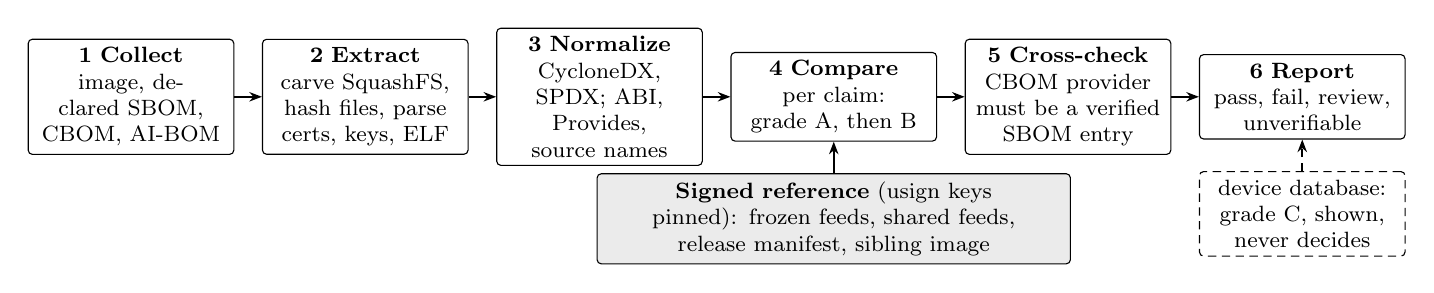
\begin{tikzpicture}[font=\footnotesize, node distance=3.5mm,
  box/.style={draw, rounded corners=1.5pt, align=center, inner sep=3pt, minimum height=9mm, text width=24mm},
  trust/.style={box, fill=black!8}, arr/.style={-{Stealth[length=1.6mm]}, semithick}]
\node[box] (obj) {\textbf{1 Collect}\\image, declared SBOM, CBOM, AI-BOM};
\node[box, right=of obj] (unp) {\textbf{2 Extract}\\carve SquashFS, hash files, parse certs, keys, ELF};
\node[box, right=of unp] (norm) {\textbf{3 Normalize}\\CycloneDX, SPDX; ABI, Provides, source names};
\node[box, right=of norm] (cmp) {\textbf{4 Compare}\\per claim: grade A, then B};
\node[box, right=of cmp] (x) {\textbf{5 Cross-check}\\CBOM provider must be a verified SBOM entry};
\node[box, right=of x] (rep) {\textbf{6 Report}\\pass, fail, review, unverifiable};
\node[trust, below=4mm of cmp, text width=58mm] (ref) {\textbf{Signed reference} (usign keys pinned): frozen feeds, shared feeds, release manifest, sibling image};
\node[box, below=4mm of rep, densely dashed, text width=24mm] (db) {device database: grade C, shown, never decides};
\draw[arr] (obj) -- (unp); \draw[arr] (unp) -- (norm); \draw[arr] (norm) -- (cmp); \draw[arr] (cmp) -- (x); \draw[arr] (x) -- (rep);
\draw[arr] (ref) -- (cmp); \draw[arr, densely dashed] (db) -- (rep);
\end{tikzpicture}
\caption{The \tool{} pipeline. Nothing from the firmware is executed. The grey box is the only trusted input.}
\label{fig:pipeline}
\end{figure*}

Figure~\ref{fig:pipeline} shows the six stages; they map onto the SafeIoT pipeline's four directories (analysis object, preprocess, security analysis, analysis output).

\textbf{Input.} Declared BOMs are read as CycloneDX \cite{cyclonedx} or SPDX JSON; names are reconciled through ABI suffixes, \texttt{Provides} aliases and source package names, so OpenWrt's published BOMs verify unchanged.

\textbf{Extraction.} The SquashFS root filesystem is carved by superblock magic and read in pure Python. Every regular file is hashed. OpenWrt binaries have no section headers, so SONAMEs are read from the dynamic segment. Certificates and keys (X.509, usign, PEM, OpenSSH, Dropbear) are parsed.

\textbf{Reference.} For a release and target the tool fetches the target's \texttt{sha256sums}, verifies its usign (Ed25519) signature against pinned keys, and from it pins the frozen package indexes, the image list and the release manifest; shared feed indexes carry their own signatures. Each package is hashed against its index entry and reduced to a per-file SHA-256 manifest. A file-path index (\indexPkgsMin{} to \indexPkgsMax{} packages per target) maps any path to candidate packages. There are four sources because OpenWrt's \emph{shared} feeds are one directory for all point releases of a series and are rebuilt after release: identical bytes get new labels and rebuilt packages get new bytes. \emph{Frozen} per-target feeds never change. The signed \emph{manifest} pins release-time labels. A \emph{sibling snapshot}, the file hashes and package list of another official image of the same release and target, restores the bytes the release was built from.

\begin{table}[t]
\caption{Evidence grades.}
\label{tab:grades}
\small
\begin{tabular}{@{}lp{0.62\columnwidth}l@{}}
\toprule
Grade & Evidence & Decides? \\
\midrule
A & every file byte-identical to the publisher's package (signed index, per-file SHA-256); label from a frozen feed, the manifest or a sibling & yes \\
B & intrinsic to the bytes: the version marker the reference build carries, SONAMEs, algorithm names & if no A \\
C & the device's own package database & never \\
\bottomrule
\end{tabular}
\end{table}

\textbf{Verdicts and triage.} Each declared component gets one verdict from the strongest evidence available (Table~\ref{tab:grades}).
\emph{Automatic pass}: \vd{verified\_A}, \vd{verified\_B}.
\emph{Automatic fail}: \vd{wrong\_version} (bytes are a build the reference labels differently), \vd{wrong\_component}, \vd{absent}, and per image \vd{undeclared\_component} (files byte-identical to a package the BOM omits) and \vd{undeclared\_file} (an executable nothing explains).
\emph{Needs a person}: \vd{bytes\_differ} (same label, different bytes: a rebuild or a modification) and \vd{label\_unconfirmed} (same bytes, nothing pins the label).
\emph{Unverifiable}: metadata packages with no files, and components whose reference has moved on and whose files carry no marker.
One harmless difference is recognised automatically: BusyBox embeds its build time, so a rebuilt copy differs in a few bytes inside date strings; these are masked before comparison. Without that rule clean-image false alarms double (\cleanFpNoNorm{} against \cleanAlarms{}).

\textbf{CBOM and cross-BOM.} Certificates and keys are compared field by field with the CBOM. Algorithms are found as narrowly matched names in each component's files (grade B). The cross-BOM rules tie the two documents together: a declared algorithm must name a providing component that is in the SBOM (\vd{provider\_not\_in\_sbom}), whose bytes verified (\vd{provider\_unverified}) and one of whose files carries the algorithm's name (\vd{algorithm\_not\_evidenced}); a component whose files name algorithms must have CBOM entries. Weak keys, expired certificates, deprecated primitives and embedded private keys are reported as policy observations. Appendix~\ref{app:taxonomy} maps these to the track's taxonomy.

\textbf{AI-BOM.} Model files are found by magic bytes (GGUF, TensorFlow Lite, ONNX, safetensors, PyTorch, HDF5) and matched to declared models by SHA-256. That is the whole scope. Routers carry no models, so this part is exercised only by synthetic unit-test fixtures and we report no accuracy for it.

\textbf{A worked example.} The repository's pipeline harness verifies one official image against a declared BOM with four seeded SBOM errors and two seeded CBOM errors. Table~\ref{tab:example} is taken from its committed report. Of \exDeclared{} declared components, \exPass{} pass automatically, \exFail{} fail, \exReview{} need review and \exUnver{} are unverifiable; all \exFilesAccounted{} of \exFiles{} files are accounted for. The two cross-BOM rows are consequences the seeding did not list: once BusyBox and Dropbear are not the declared builds, the CBOM's statements about what they provide are no longer supported. The report also lists \exDeprecated{} deprecated-primitive observations (MD5, SHA-1, RC4, 3DES, WEP, TKIP named in binaries) and, in a separate section, the \exDbDisagree{} places where the device database disagrees with the BOM, labelled grade C.

\begin{table*}[t]
\caption{Findings \tool{} reports on the repository's example: one official image, a declared BOM with seeded errors. Generated from the committed report.}
\label{tab:example}
\footnotesize
\begin{tabular}{@{}lllcl@{}}
\toprule
BOM & Finding & Subject & Grade & Evidence \\
\midrule
\tabexamplerows
\bottomrule
\end{tabular}
\end{table*}

\section{Evaluation}
\label{sec:eval}

\begin{table*}[t]
\caption{Held-out images: precision / recall on \nHeldCases{} seeded single-error cases. The three \tool{} columns add reference sources from left to right; the two left ones are the conservative reading (\S\ref{sec:easy}). ``n/a'': the tool reported nothing.}
\label{tab:main}
\small
\begin{tabular}{@{}lr ccc ccc@{}}
\toprule
 & & \multicolumn{3}{c}{\tool{}, reference sources used} & \multicolumn{3}{c}{Baselines} \\
\cmidrule(lr){3-5}\cmidrule(lr){6-8}
Device database & Cases & signed feeds only & + signed manifest & + sibling (default) & BomTrace & Syft-diff & cve-bin-tool-diff \\
\midrule
\tabmainrows
\bottomrule
\end{tabular}
\end{table*}

\subsection{Setup}

\textbf{Data.} \nImages{} official OpenWrt release images (23.05.6 and 24.10.8) over \nArchAll{} package architectures: MIPS big and little endian, AArch64, ARMv7 and x86-64 \cite{openwrt}. Images are fetched and checked against signed release metadata, never redistributed.
\textbf{Split.} \nTuneImages{} tuning images were used to write and debug the rules. The \nHeldImages{} held-out images (\nArchHeld{} architectures) were not verified until the rules were frozen at commit \texttt{\freezeCommit}; the full run was started from that commit with a clean tree. Later changes touch no benchmark rule, and a rerun of \postImages{} images (\postCases{} cases) shows \postDiffs{} score differences.
\textbf{Ground truth.} The correct BOM of an unmodified official image is its package list. Each case applies one mutation with one label (Appendix~\ref{app:classes}): M1 omitted component, M2 version of the other release series, M2b fabricated version, M3 phantom component, M4 and M4u implanted package, M5 binary swapped for another release's build, M6 one byte flipped; \kPerClass{} seeded targets per class per image (\kUnindexed{} for M4u, seed \seed).
\textbf{Database conditions.} For M1 to M3 the device database is \emph{honest} (untouched), \emph{colluding} (edited to agree with the wrong BOM) or \emph{stripped} (deleted). M4 to M6 are \emph{unaware}: neither BOM nor database mentions the change. The first three rows of Table~\ref{tab:main} are the same \nBomErrCases{} cases in three database states, not independent samples.
\textbf{Baselines.} BomTrace's published verifier, unmodified, at commit \texttt{\bomtraceCommit}; \emph{Syft-diff}, Syft~1.57.2's inventory compared with the BOM by a script of ours; \emph{cve-bin-tool-diff}, the version scanner of cve-bin-tool~3.4 likewise. Syft and cve-bin-tool are not verifiers; the diffs are ours.
\textbf{No manual expert review} was used as a baseline; ground truth is by construction.
\textbf{Scoring.} Recall is labelled errors found over labelled errors; an undeclared component must be named. Precision is $TP/(TP+FP)$ where $FP$ includes every finding on the unmodified image with the correct BOM, counted once per image, plus findings a mutation caused beyond its label.

\subsection{Database dependence}

Table~\ref{tab:main} gives the result. Read the baselines down the rows: BomTrace goes from \rHonBt{} recall with an honest database to \rColBt{} with a colluding or stripped one, and Syft-diff from \rHonSy{} to \rColSy{} and \rStrSy{} (in the stripped condition it reports every declared component as absent, which credits it with the phantom cases at precision \pStrSy). Neither finds any of the \nUnawareCases{} implanted, swapped or patched binaries. This is the designed behaviour of those tools and their documentation predicts it; we show it so the dependence is measured and not asserted. cve-bin-tool-diff is independent of the database but covers few components. Syft-diff's low precision with an honest database comes from \syftCleanMin{} to \syftCleanMax{} naming differences per clean image in our diff script, not from Syft.

\tool{} gives identical answers in the first three rows because it never reads the database. With signed feeds only: precision \pColFo, recall \rColFo{} (95\% Wilson interval \loColFo{} to \hiColFo; lowest single image \minColFo). Adding the signed manifest: \pColNs{} / \rColNs{} (\loColNs{} to \hiColNs). Adding a sibling snapshot: \pColBw{} / \rColBw{} (\loColBw{} to \hiColBw). On the unaware cases recall is \rUnaFo{} without and \rUnaBw{} with the snapshot. The tools are complementary: when the database happens to be honest, showing its disagreements as grade C evidence lifts \tool{} to \tpHonWithDb{} of \nBomErrCases.

\subsection{Is this easy by construction?}
\label{sec:easy}

Largely yes, and three facts bound how much.

\emph{The sibling is a twin.} Of the \nImages{} images, \sibHave{} have a sibling of the same target; for \sibTwins{} of those the sibling's root filesystem is byte-identical to the tested image's, and the other \sibRest{} share \sibRestMinPct\% to \sibRestMaxPct\% of files. The snapshot is therefore the publisher's frozen release filesystem, not an independent witness. It is the right reference for auditing vendor firmware built from a release, but for this benchmark it nearly hands over the answer. That is why Table~\ref{tab:main} leads with the columns that do not use it. Replacing each sibling by the least similar one on the \farImages{} held-out images that have one changes little (colluding recall \farColR, unaware \farUnaR).

\emph{Without the twin the task is not trivial.} With feeds only, half of the fabricated versions go unrefuted (\kMTwoBFo{} of \kMTwoBCases{} found): on identical bytes, a label that differs from a shared feed's cannot be told from the feed's own relabelling, so the verdict is \vd{label\_unconfirmed} and not a failure. The signed manifest recovers most of them (\kMTwoBNs). Even a one-byte patch goes unreported \emph{without} the snapshot in \patchMissNoSnap{} of \kMSixCases{} cases: all are in ucode and LuCI packages whose shared-feed copy has since moved to a newer version, which leaves no same-version reference to differ from.

\emph{Official images against their own publisher's packages are the favourable case.} Grade A needs the builder's signed binaries. \S\ref{sec:fork} shows what is left without them.

Grade B alone (version markers, no hashes) reaches recall \rColBo{} on BOM-level errors and \rUnaBo{} on unaware cases, which is the realistic ceiling when no byte-identical reference exists.

\subsection{Reference drift}
\label{sec:drift}

\begin{figure}[t]
\centering
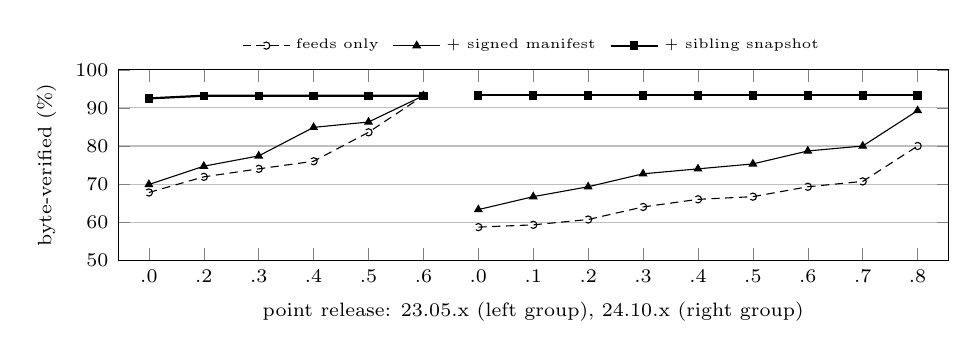
\begin{tikzpicture}
\begin{axis}[width=\columnwidth, height=40mm, symbolic x coords/.expand once={\driftticks}, xtick/.expand once={\driftticks}, xticklabels/.expand once={\driftticklabels}, enlarge x limits=0.04,
  x tick label style={font=\scriptsize}, y tick label style={font=\scriptsize},
  xlabel={\scriptsize point release: 23.05.x (left group), 24.10.x (right group)},
  ymin=50, ymax=100, ytick={50,60,70,80,90,100}, ylabel={\scriptsize byte-verified (\%)}, ymajorgrids,
  legend style={font=\tiny, at={(0.5,1.03)}, anchor=south, legend columns=3, draw=none, /tikz/every even column/.append style={column sep=3pt}}]
\driftplots
\end{axis}
\end{tikzpicture}
\caption{Share of a correct BOM confirmed byte for byte against today's reference, same device, \driftReleases{} point releases.}
\label{fig:drift}
\end{figure}

How long does a public reference stay usable? We verified a correct BOM for the same device across \driftReleases{} point releases against today's feeds (Figure~\ref{fig:drift}). For 24.10.0 (\driftOldTwentyFourAge{} days old) the shared feed alone confirms \driftOldTwentyFourFo\% of components byte for byte and raises \driftOldTwentyFourFoAlarms{} false alarms; \driftOldTwentyFourRelabelled{} of \driftOldTwentyFourDeclared{} components have a changed feed label. The manifest lifts that to \driftOldTwentyFourMa\%, a sibling snapshot to \driftOldTwentyFourSn\% with \driftOldTwentyFourSnAlarms{} alarms. Even the newest release, 24.10.8 (\driftNewTwentyFourAge{} days), is at \driftNewTwentyFourFo\% from feeds alone: \republishedTwentyFourPct\% of the 24.10 base feed was republished after that release was built. Drift follows feed activity, not age: 23.05.6 is \driftNewTwentyThreeAge{} days old and fully covered (\driftNewTwentyThreeFo\%), with \republishedTwentyThreePct\% of its base feed republished. Over all \driftReleases{} releases the feeds alone raise \driftFeedAlarmsTotal{} false alarms and the snapshot configuration \driftSnapAlarmsTotal. The lesson for anyone verifying BOMs after the fact: archive the release bytes, or a per-file hash manifest, at release time. A mutable package feed is not a durable reference.

\subsection{OpenWrt's published BOMs}

OpenWrt publishes one CycloneDX BOM per target. We verified them unchanged against the \obImages{} device images: \obVerified{} of \obClaims{} claims verify, \obUnverifiable{} are unverifiable (mostly packages without files), and \obWrongVersion{} version claims on \obWrongVersionImages{} images are contradicted by the bytes. All \obWrongVersion{} follow one pattern: wireless kernel-module packages built out of tree (cfg80211 and mac80211 backports, ath and mt76 drivers) are listed with the kernel's version only, while the bytes are the build the frozen feed labels with the kernel and the driver version. \obAbsent{} listed components are not in the device image, and \obBeyondImages{} images carry packages the per-target BOM does not list (\obBeyondMin{} to \obBeyondMax{} per image, \obBeyondTotal{} in total), mainly device-specific kernel modules (Wi-Fi, USB, Ethernet, crypto) and firmware blobs. We found no statement that the per-target BOM is meant to describe each device image, so we report this as a coverage observation, not a defect. It is not synthetic, and a database-reading verifier and a byte-level one both find it; ours additionally confirms that the remaining claims are the publisher's bytes.

\subsection{Case study: an unmodified downstream fork}
\label{sec:fork}

Vendor firmware is usually a rebuild. As a stand-in we took an unmodified ImmortalWrt \forkRelease{} image for one benchmark device \cite{immortalwrt}, with its own package list as the declared BOM. Verified against \emph{upstream} OpenWrt, only \forkUpVerA{} of \forkDeclared{} components (\forkUpVerAPct\%) are upstream's bytes, \forkExeSame{} of \forkExeTotal{} executables match the upstream image, and the report has \forkUpWrongVersion{} \vd{wrong\_version}, \forkUpBytesDiffer{} \vd{bytes\_differ} and \forkUpOrphans{} unexplained executables. None of that indicates tampering; it is what a rebuild looks like. Verified against the fork's \emph{own} signed download tree, with a different key and no code change, \forkOwnVerified{} of \forkDeclared{} verify with \forkOwnFindings{} findings, and all \forkOmittedFound{} of \forkOmitted{} omitted components are found in every database condition. So the method transfers to a second publisher, and grade A is available exactly when the builder publishes signed binaries or per-file manifests. That is a requirement worth writing into procurement.

\subsection{Errors, false alarms, CBOM and cost}

\textbf{Clean images.} On the held-out images with correct BOMs, \cleanVerA{} of \cleanDeclared{} components verify byte for byte (\cleanVerAPct\%), \cleanVerB{} by marker, \cleanUnver{} are unverifiable (\cleanUnverMeta{} are packages without files) and \cleanAlarms{} are false alarms (\cleanAlarmPct\%). In triage terms: \cleanPassPct\% automatic pass, \cleanAlarmPct\% review, \cleanUnverPct\% unverifiable. All \cleanAlarms{} are \vd{bytes\_differ} on \texttt{e2fsprogs} on single-device targets with no sibling: the image's build differs from the feed's under the same label, and the tool cannot say which is the odd one. \cleanAccounted{} of \cleanFiles{} files and all \cleanCode{} executables are accounted for.
\textbf{Misses.} The default configuration misses \nMisses{} cases and has \caseFp{} case-level false positives. \missImplant{} are implants from the large \texttt{packages} feed, which the default index omits: each was flagged as unexplained executable code but not named, which we count as a miss. Indexing that feed (\wideMbMin{} to \wideMbMax{}~MB more per architecture) names \wideAfter{} of \wideCases{} on \wideImages{} images instead of \wideBefore. \missPhantom{} phantom packages were accepted because the image holds one of their files, a script another installed package ships with identical bytes; requiring a package's executables would catch them, but we did not change rules after the freeze. \missFabricated{} fabricated versions slipped through, one \emph{confirmed} at grade B by a coincidental version string, a reminder that a marker is weaker than a hash.
\textbf{CBOM.} On \cbomCases{} seeded cases in \cbomClasses{} classes the checks produce \cbomTp{} of \cbomExpected{} expected findings and \cbomExtra{} extra. The correct CBOM comes from the same detector, so this shows that the rules are consistent, not that the detector finds all cryptography.
\textbf{Inventory.} From bytes alone, with no BOM and no database, \tool{} names \invNamed{} of \invInstalled{} installed packages with \invWrong{} wrong names; on the same trees Syft lists \invSyftMin{} to \invSyftMax{} components.
\textbf{Cost.} A verification takes \secMin{} to \secMax{}~s with a warm cache (BomTrace \secBomtrace~s, Syft \secSyft~s). Building the reference for one release and target takes \indexSecMin{} to \indexSecMax{}~s and \indexMbMin{} to \indexMbMax{}~MB once.

\section{Impact and Pipeline Fit}

\emph{Manufacturers} can run \tool{} in release CI to catch a BOM generated from the wrong build before it ships. \emph{Auditors and buyers} get a report whose every line says which evidence supports it and how strong that evidence is, and an explicit list of what could not be checked. \emph{Regulators} get a concrete, testable requirement: a BOM is verifiable to grade A only if the builder publishes signed per-file reference material. The repository mirrors the SafeIoT pipeline layout with a harness that goes from a clean checkout to a checked result in under a minute, exits non-zero on findings, and reruns as feeds change. The method is not specific to routers: any firmware whose components come from a signed binary distribution (Debian-based cameras and gateways, Yocto or Buildroot products with published package feeds) fits the same reference interface; devices built entirely in-house fall back to grade B. The benchmark, the seeded-error generator, the three baseline adapters and all result files are reusable.

\section{Limitations}

\textbf{One firmware family.} All measurements are on official OpenWrt opkg releases; apk-based 25.12 is unsupported.
\textbf{Seeded errors are not field data.} The numbers describe behaviour on eight defined error classes, not real-world BOM error rates. Statically linked code inside another binary is outside every class.
\textbf{Proprietary and rebuilt components} have no public reference; they end as \vd{unverifiable} or \vd{bytes\_differ} (\S\ref{sec:fork}).
\textbf{Encrypted or unrecognised images} cannot be unpacked; only the SquashFS root filesystem is analysed, not the kernel image or boot loader.
\textbf{Stripped binaries} leave grade A intact (hashes do not need symbols) but weaken grade B.
\textbf{\vd{bytes\_differ} needs a person:} a patch and a harmless rebuild look the same to a hash.
\textbf{The reference drifts} (\S\ref{sec:drift}), and \textbf{the trust anchor} is two pinned keys; a compromised publisher makes every verdict wrong.
\textbf{CBOM evidence is string-level,} from a hand-written table of \nAlgPatterns{} patterns; an unnamed implementation is missed and a name is not proof of use.
\textbf{AI-BOM is a presence check} with no evaluation.
\textbf{Not covered:} vulnerability matching, licences, provenance fields and documentation.
\textbf{Baselines} run outside their stated scope in two conditions; the comparison shows a dependency, not a ranking.

\section{Conclusion}

A BOM checked against the firmware's own package database is checked against a second copy of the same claim. Verifying against the publisher's signed bytes removes that dependence and makes swapped and patched binaries visible, at the price of needing a reference that someone published and preserved. The benchmark numbers are high because the method is simple; the results we would stress are the measured blind spot of database-reading verification, the decay of mutable feeds, the errors in real published BOMs, and the honest remainder that no tool can verify without the builder's help.

\begin{acks}
This project was built and written with AI coding agents working under the author's direction: the code, experiments, analysis and text were produced with their assistance. The author is responsible for the content. Every number in this paper is generated from a committed result file and checked against the PDF by a script in the repository (\texttt{paper/check\_numbers.py}). Code, benchmark and results: \url{https://github.com/awinton64/bomwitness} (MIT).
\end{acks}

\bibliographystyle{ACM-Reference-Format}
\bibliography{refs}

\appendix

\section{Verification Taxonomy}
\label{app:taxonomy}

\begin{table}[H]
\caption{The track's taxonomy and what \tool{} does with each item.}
\small
\begin{tabular}{@{}p{0.34\columnwidth}p{0.40\columnwidth}l@{}}
\toprule
Track item & Finding & Tier \\
\midrule
missing software component & \vd{undeclared\_component}, \vd{undeclared\_file} & auto \\
incorrect component version & \vd{wrong\_version}; \vd{label\_unconfirmed} & auto; review \\
undeclared dependency & as undeclared component; dependency edges are not checked & partly \\
vulnerable component & not covered (a note when the feed ships a newer version) & none \\
deprecated cryptographic primitive & \vd{deprecated\_algorithm}, \vd{deprecated\_signature\_hash} & auto (B) \\
weak key size & \vd{weak\_key}, \vd{wrong\_key} & auto \\
expired or self-signed certificate & \vd{expired\_certificate}, \vd{wrong\_expiry}; self-signed is recorded & auto \\
missing AI model metadata & \vd{undeclared\_model}, \vd{absent\_model} (presence only) & partly \\
inconsistent AI model/runtime dependency & not covered & none \\
unverifiable provenance claim & \vd{unverifiable}, \vd{bytes\_differ}; supplier fields not checked & review \\
wrong or missing license information & not covered & none \\
\bottomrule
\end{tabular}
\end{table}

\section{Recall by Error Class}
\label{app:classes}

\begin{table}[H]
\caption{Held-out cases found per class. \tool{} columns: feeds only (F), + manifest (M), + snapshot (S). Baselines: honest / colluding / stripped database, or the unaware condition.}
\footnotesize
\setlength{\tabcolsep}{2.5pt}
\begin{tabular}{@{}lp{0.25\columnwidth}r rrr ccc@{}}
\toprule
 & Class & $n$ & F & M & S & BomTrace & Syft-diff & cve-bin \\
\midrule
\tabclassrows
\bottomrule
\end{tabular}
\end{table}

\section{Held-out Images}

\begin{table}[H]
\caption{Clean controls per held-out image (correct BOM, default configuration): declared components, verified at grade A and B, unverifiable, needing review, and how close the sibling used for the snapshot is (share of identical files).}
\footnotesize
\setlength{\tabcolsep}{1.8pt}
\begin{tabular}{@{}lll rrrrr l@{}}
\toprule
Device & Rel. & Architecture & Decl. & A & B & Unv. & Rev. & Sibling \\
\midrule
\tabimagerows
\bottomrule
\end{tabular}
\end{table}

\section{Reproducing}

\texttt{pip install -e ".[test]"} and \texttt{pytest} run the offline unit tests on a synthetic signed feed. The harness script \vd{pipeline/\allowbreak pipeline\_harness/\allowbreak bomwitness/\allowbreak run.sh} verifies one official image end to end. The file \vd{docs/\allowbreak EVALUATION.md} lists the commands for the full benchmark, the baselines and each measurement; \vd{results/r2/} holds every result file. The public repository is a single-commit export of the development history, so the commit ids quoted in this paper refer to that history; \vd{docs/\allowbreak PROVENANCE.md} lists it together with the rule files that changed after the freeze. Shared feeds keep moving, so a later rerun of the feed-dependent columns and of Figure~\ref{fig:drift} will show more drift; frozen feeds, manifests and images do not change.

\end{document}
